\section{Modelling the Game}

% what this section talks about
%   - graph of objects and relations
%   - what each model object represents and is
%   - difficulties developing the model
%   - model: sector, game, entity, ship, plan, goal, ship action, ship class, ship configuration, weapon, system, weapon slot, system slot, fleet, Formation, client state
% what is a game model
% early on
% 

This section describe the model that makes the game.
The model describes the different concepts in the game, for instance a weapon, a ship, a formation, etc.
It also describes the relationships between them, for instance a ship has many weapons.
Initially, the game model was simple, but as the design stage progressed, the game model gained complexity.

% sector
The game's terrain is called a sector. The sector has the following fields:
\begin{margintable}
    \begin{tabular}{p{4em} p{11em}}
    \toprule
    \emph{fields} & \emph{description} \\
    \midrule

    name & name of sector \\
    size & size of game \\
    spawn points & the points on the sector where player's fleets are spawned \\
    planets & all the planets in the sector \\
    space lanes & the spaces lanes connecting all the planes \\

    \bottomrule
    \end{tabular}
    	\vspace{1em}
	\caption{sector layout}
	\label{tab:model:sectorFields}
\end{margintable}

A sector is basically a game map.
It specifies the layout of the map, it contains fields that are described in Table \ref{tab:model:sectorFields}.

When the player starts the game, they are able to choose which sector they want to play by its name. 
The spawn points on the sector are typically as far apart as possible. 
This means that bigger sector will typically have longer playing periods relative to smaller sectors.
The sector specifies which planets are includes as well as which planets are connected by space lanes as shown in Figure \ref{fig:model:sectorRelation}

\begin{marginfigure}
	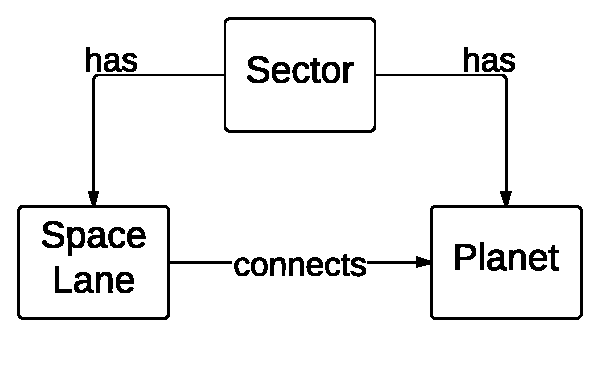
\includegraphics{res/model/sector.pdf}
	\caption{relationship between setor, planet, and space lanes}
	\label{fig:model:sectorRelation}
\end{marginfigure}

% planet
Planets in the sector have a variety of properties that make the planet unique.
Table \ref{tab:model:planetFields} gives a breakdown of the planet's properties.

\begin{margintable}
    \begin{tabular}{p{4em} p{11em}}
    \toprule
    \emph{Fields} & \emph{Description} \\
    \midrule
    name & name of planet, used for identifying planets \\
    ecotype & type of planet, eg star, ocean, metal, etc \\
    location & location of planet within the sector \\
    resources & the quantity of resources generated by this planet if captured\\
    \bottomrule
    \end{tabular}
    	\vspace{1em}
	\caption{sector layout}
	\label{tab:model:planetFields}
\end{margintable}

The planet's name is a colloquial name used by players to reference a specify planet.
There a variety of planet ecotypes, some examples shown in Figure \ref{fig:model:starPlanet}, \ref{fig:model:oceanPlanet}, and \ref{fig:model:metalPlanet}.
The ecotype of a planet effects its appearance as well as its distribution of resources.
Some ecotypes will typically have a greater proportion of say metal relative to fuel and anti-matter, whilst another ecotype may favour fuel.

% TODO fix margin diagrams, all appearing below the page (invisible)
\begin{marginfigure}
	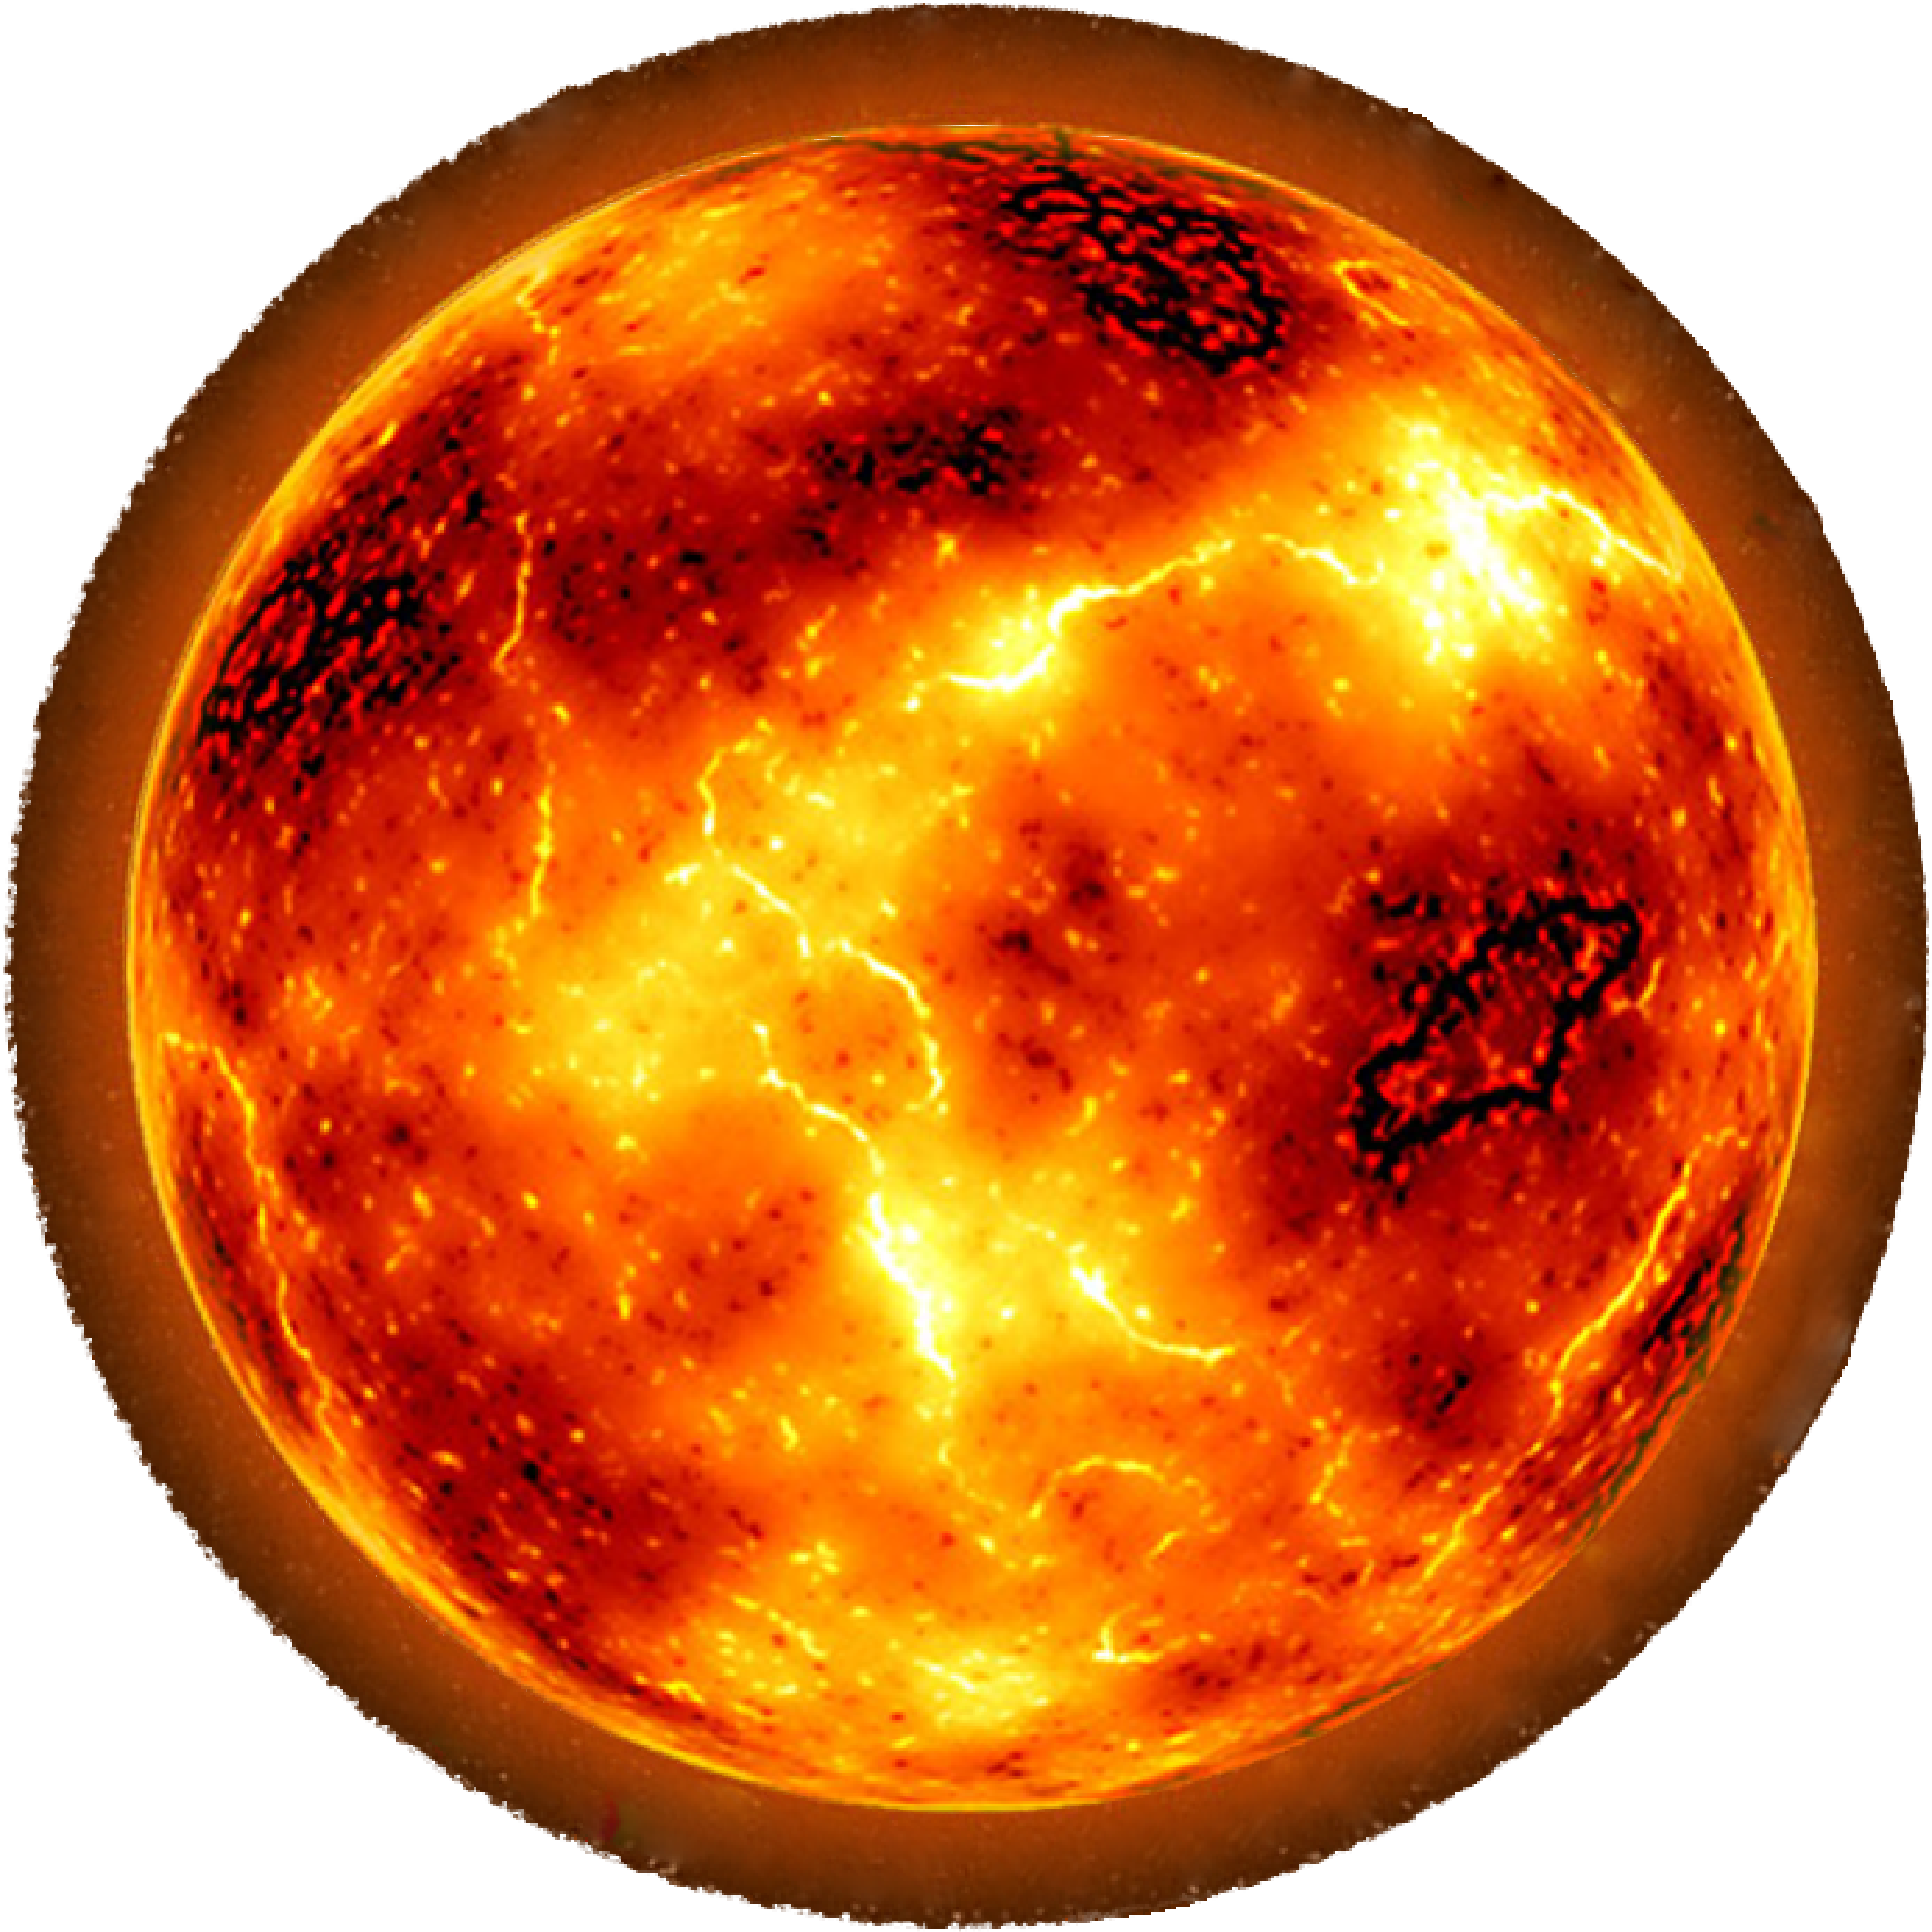
\includegraphics{res/planets/star.png}
	\caption{ecotype: star}
	\label{fig:model:starPlanet}
\end{marginfigure}

\begin{marginfigure}
	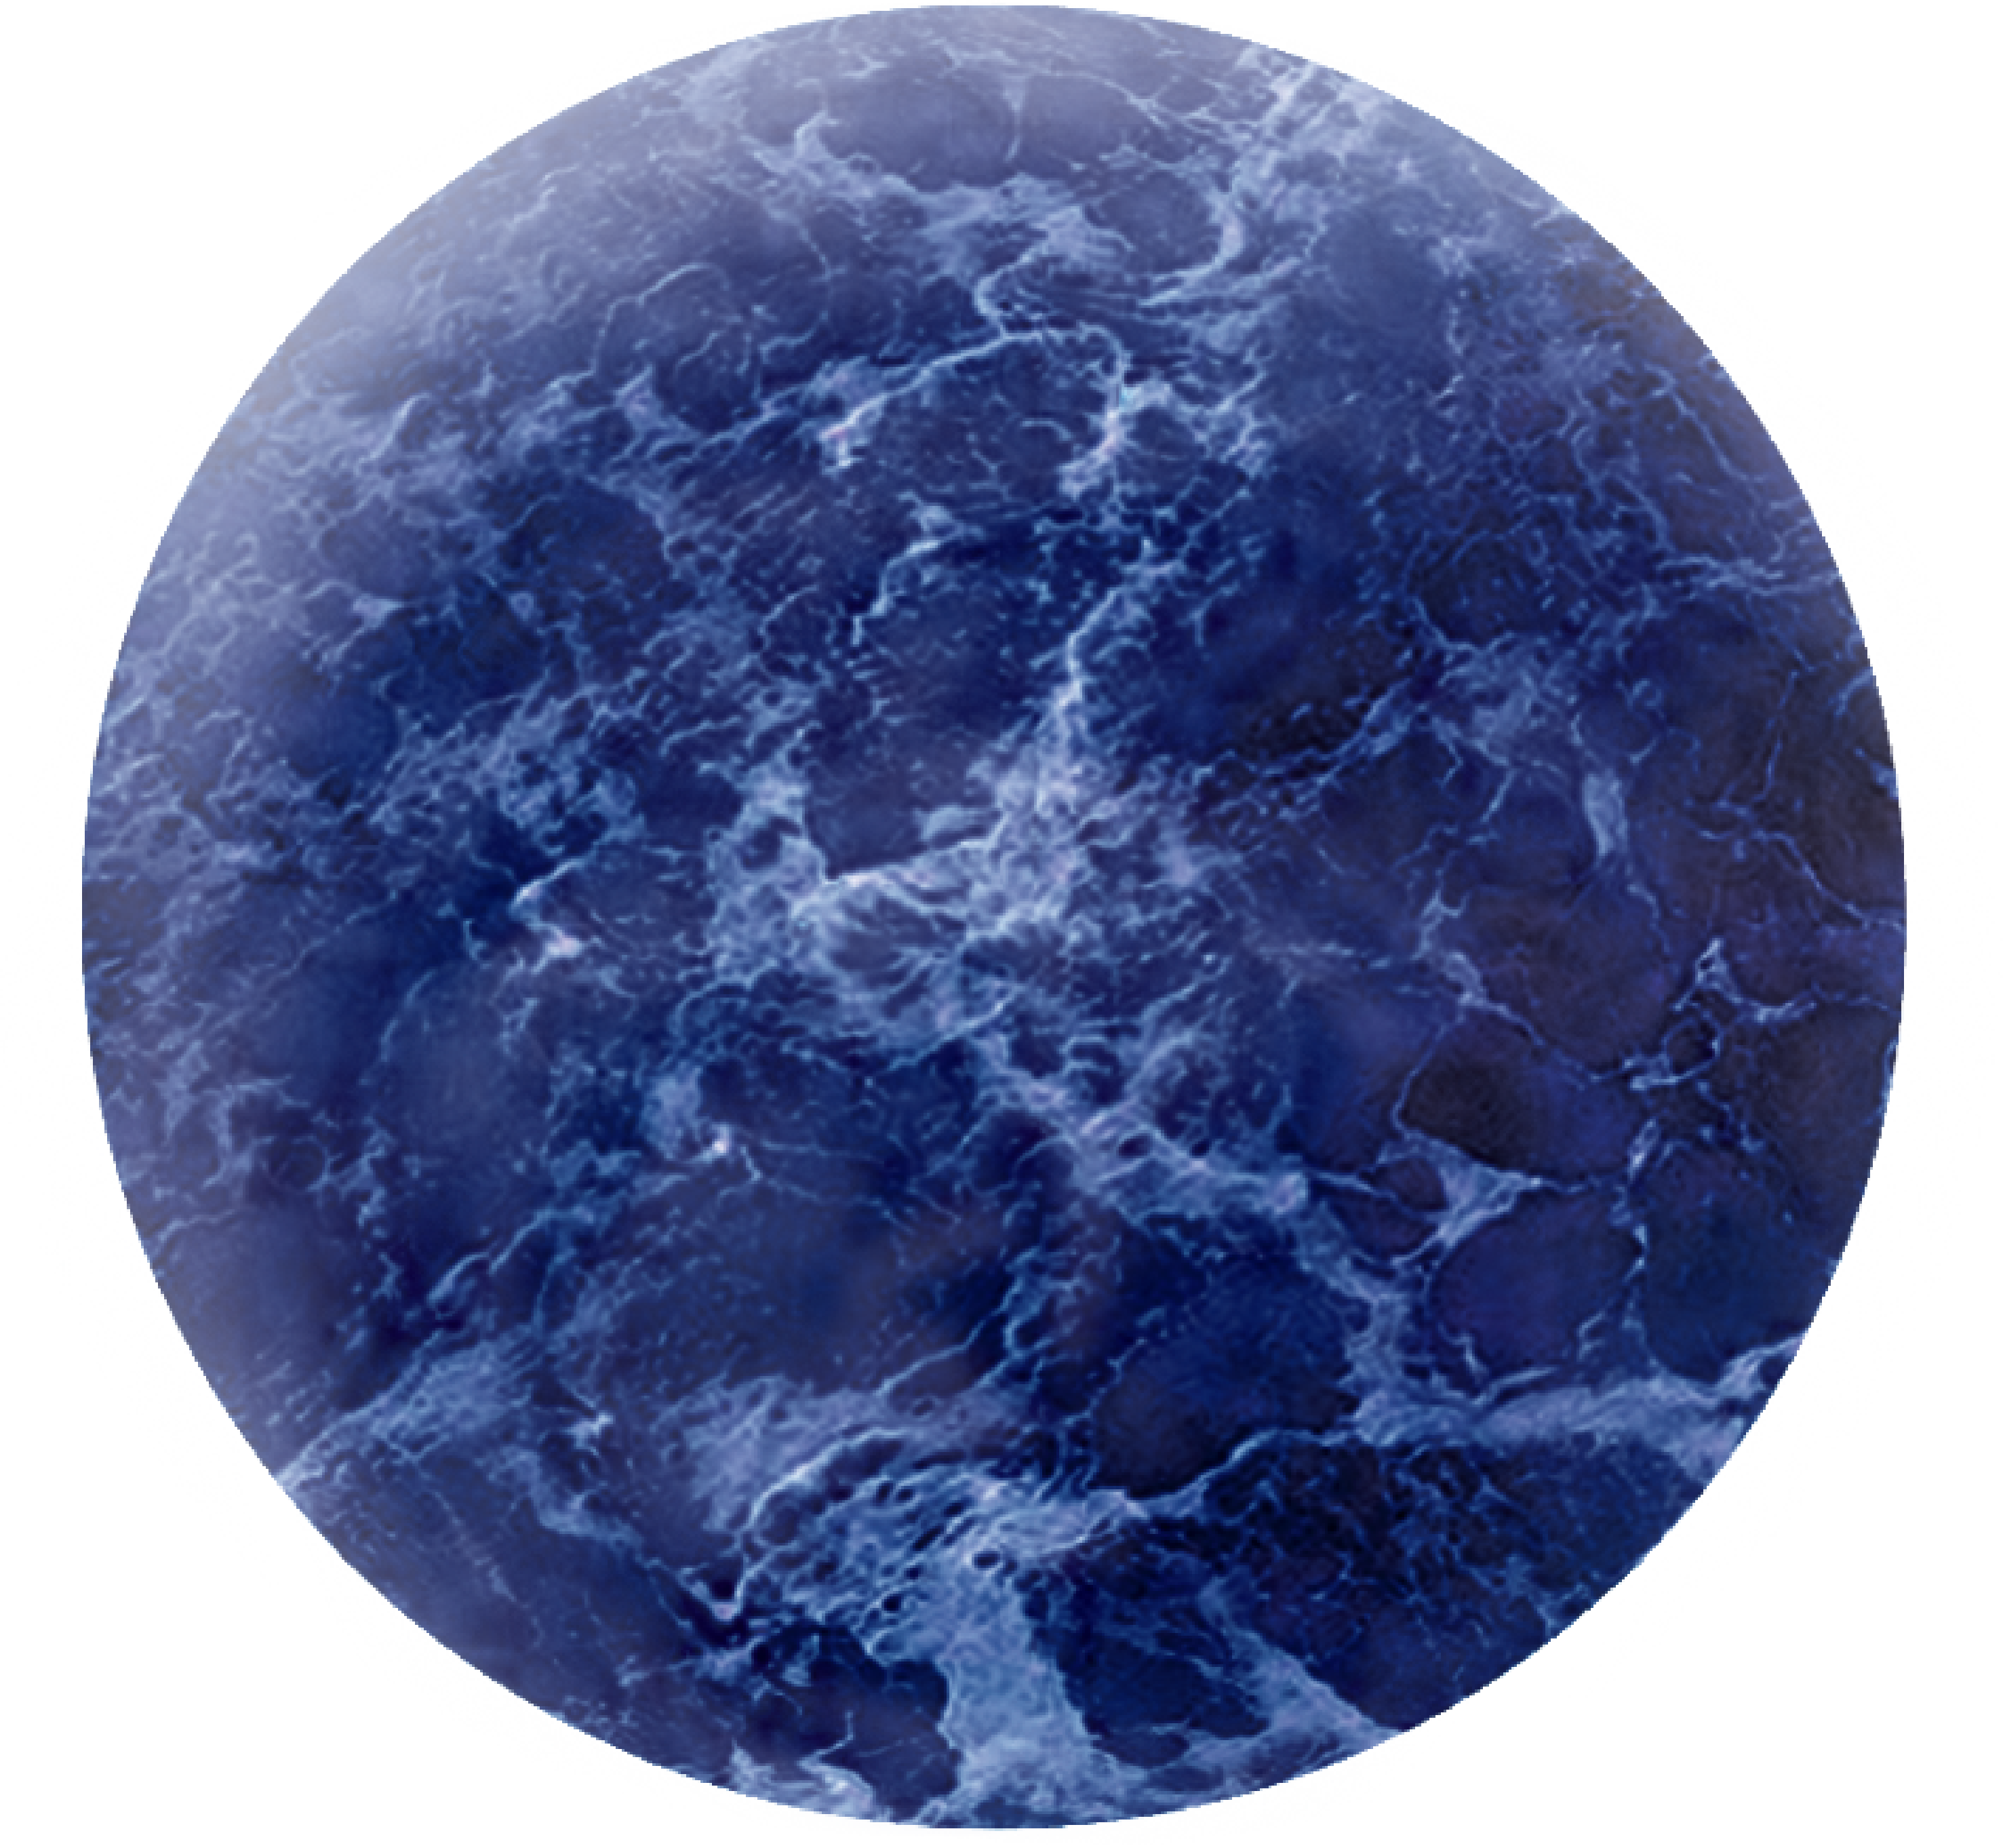
\includegraphics{res/planets/OceanPlanet.png}
	\caption{ecotype: ocean}
	\label{fig:model:oceanPlanet}
\end{marginfigure}

\begin{marginfigure}
	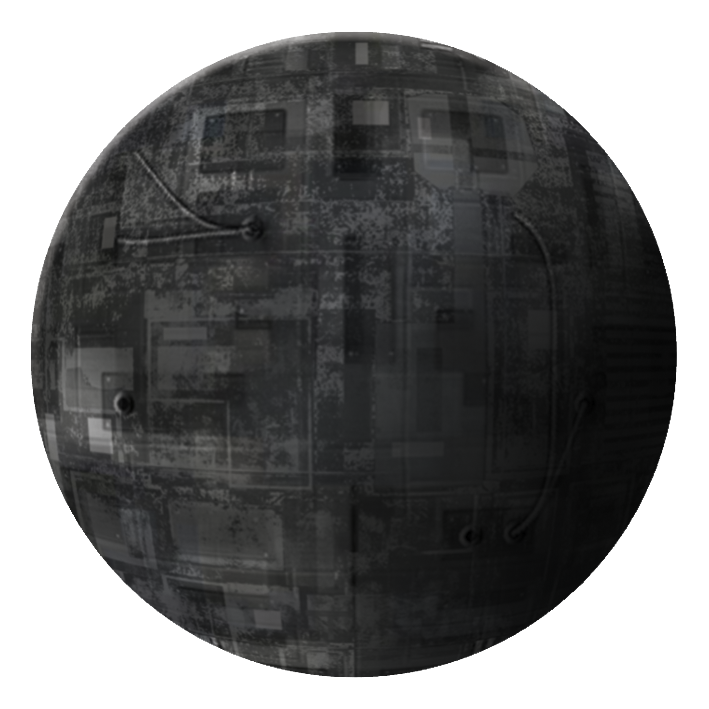
\includegraphics{res/planets/metal-planet.png}
	\caption{ecotype: metal}
	\label{fig:model:metalPlanet}
\end{marginfigure}


% space lanes
A Space Lane can be harnessed by ships to travel between planets incredible fast.
Each sector will have its own Space Lanes unique to that Sector.


% ship
The ship part of the model is actually broken down into 3 key concepts: Ship, Ship Configuration and Ship Class.
The Ship Class represents the the hull of the ship, its size, number of weapon sots etc. Every ship in the game will have exactly one ship class. The Ship Configuration specifies which weapons and systems go in which slots. Figure \ref{fig:model:shipRelation} demonstrates this relation.
This distinction between Ship, Ship Configuration and Ship Class was a revised addition, because it allowed multiple ships to belong to the same class as well as being able to save the ship configuration to disk, whilst it wouldn't make sense to save a ship to disk since it only exists in that instance of the game.

% ship class
The ship class is a container that is treated as the ship's hull, but in fast it provides more information than just that, it also provides meta-data about the image being used as the ship's hull.
The image being used for the ship's hull has no meta-data attached to it, so this must be specified somewhere, and it is, in the ship class.
The reason the image needs this meta-data is because properties such as centre of rotation cannot be determined. 
They are intrinsically linked to the style of ship. 
For example take 2 images used for ship's hulls, they have identical dimensions but the first one has engines at the front of the ship so you would want the centre of rotation much closer to the front than the second one. 
Table \ref{tab:model:shipClassFields} gives a detailed description of the ship class properties.

\begin{marginfigure}
	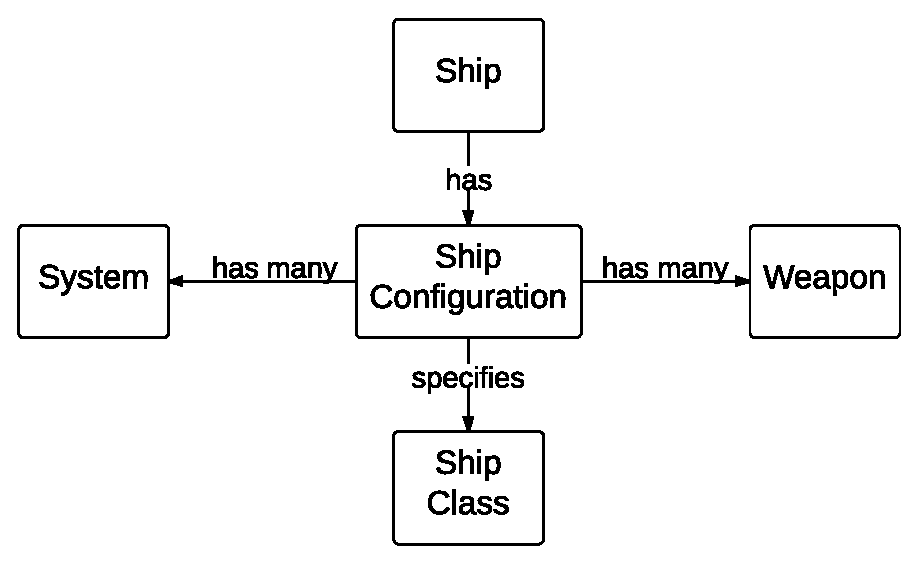
\includegraphics{res/model/ship.pdf}
	\caption{ship layout}
	\label{fig:model:shipRelation}
\end{marginfigure}

\begin{margintable}
    \begin{tabular}{p{4em} p{11em}}
    \toprule
    \emph{Fields} & \emph{Description} \\
    \midrule
    centre of rotation & point on the ship class where it rotates when turning \\
    speed & maximum speed of this hull \\
    health & health of the hull \\
    weapon slots & specifies where the weapon slots are on the hull and what type they are \\
    system slots & specifies where the system slots are on the hull \\
    name & name of the hull, used by player \\
    cost & cost of adding a ship with this hull to the fleet \\
    \bottomrule
    \end{tabular}
    	\vspace{1em}
	\caption{properties of ship class}
	\label{tab:model:shipClassFields}
\end{margintable}


% ship, ship configuration, ship class, weapons, system


% order/plan/goal


